% ============================================================
\chapter{Sous-diff\'erentiels et Sous-gradients}
\label{ch:sous_differentiels}
% ============================================================

\section{Introduction}

Voici un probl\`eme concret~: vous voulez minimiser $\norm{x}_1$ sous contraintes lin\'eaires --- un probl\`eme central en apprentissage parcimonieux. Mais la norme $\ell_1$ n'est pas diff\'erentiable \`a l'origine~: elle poss\`ede un \og coin \fg. Le gradient n'existe pas, et pourtant c'est pr\'ecis\'ement l\`a que se trouve le minimum. Comment \'ecrire une condition d'optimalit\'e sans gradient~?

La r\'eponse, d\'evelopp\'ee par Jean-Jacques Moreau et R.~Tyrrell Rockafellar dans les ann\'ees 1960, est le \emph{sous-diff\'erentiel}~: au lieu d'un unique plan tangent, on consid\`ere \emph{tous} les hyperplans qui restent en-dessous du graphe de la fonction. Aux points de diff\'erentiabilit\'e, il n'y en a qu'un (le gradient classique). Aux coins, il y en a une infinit\'e, formant un ensemble convexe compact. Cette g\'en\'eralisation ouvre la voie \`a une th\'eorie de l'optimisation non lisse d'une remarquable coh\'erence.

\begin{intuition}
Pour une fonction diff\'erentiable, le gradient d\'efinit l'unique hyperplan tangent
qui minore la fonction. Pour une fonction convexe non lisse, il peut exister
\emph{plusieurs} hyperplans minorants en un point --- leur ensemble forme le
sous-diff\'erentiel.
\end{intuition}

\section{D\'efinition du sous-gradient et du sous-diff\'erentiel}

\begin{definition}[Sous-gradient]
Soit $f : \R^n \to \R \cup \{+\infty\}$ une fonction convexe. Un vecteur
$g \in \R^n$ est un \emph{sous-gradient} de $f$ en $x \in \mathrm{dom}(f)$ si~:
\[
    f(y) \geq f(x) + \inner{g}{y - x}, \quad \forall y \in \R^n.
\]
\end{definition}

\begin{definition}[Sous-diff\'erentiel]
Le \emph{sous-diff\'erentiel} de $f$ en $x$, not\'e $\partial f(x)$, est l'ensemble
de tous les sous-gradients de $f$ en $x$~:
\[
    \partial f(x) = \{g \in \R^n \mid f(y) \geq f(x) + \inner{g}{y-x}, \; \forall y \in \R^n\}.
\]
Si $x \notin \mathrm{dom}(f)$, on pose $\partial f(x) = \emptyset$.
\end{definition}

\begin{theoreme}[Existence des sous-gradients]
\label{thm:existence_sg}
Soit $f : \R^n \to \R \cup \{+\infty\}$ convexe propre. Alors $\partial f(x) \neq \emptyset$
pour tout $x \in \mathrm{ri}(\mathrm{dom}(f))$. En particulier, si $\mathrm{dom}(f)$
est ouvert, $\partial f(x) \neq \emptyset$ pour tout $x \in \mathrm{dom}(f)$.
\end{theoreme}

\begin{proof}
Soit $x \in \mathrm{ri}(\mathrm{dom}(f))$. Le point $(x, f(x))$ est sur le bord de
$\mathrm{epi}(f)$, qui est convexe. Par le th\'eor\`eme de l'hyperplan d'appui,
il existe $(g, -\alpha) \neq 0$ tel que~:
\[
    \inner{g}{y - x} - \alpha(t - f(x)) \leq 0, \quad \forall (y,t) \in \mathrm{epi}(f).
\]
En prenant $y = x$ et $t \to +\infty$, on obtient $\alpha \geq 0$. Si $\alpha = 0$,
alors $\inner{g}{y-x} \leq 0$ pour tout $y \in \mathrm{dom}(f)$, ce qui contredit
$x \in \mathrm{ri}(\mathrm{dom}(f))$ (sauf si $g = 0$). Donc $\alpha > 0$, et
$g/\alpha$ est un sous-gradient.
\end{proof}

\section{Propri\'et\'es du sous-diff\'erentiel}

\begin{theoreme}[Propri\'et\'es fondamentales]
\label{thm:prop_subdiff}
Soit $f : \R^n \to \R \cup \{+\infty\}$ convexe propre.
\begin{enumerate}
    \item $\partial f(x)$ est un ensemble convexe ferm\'e (\'eventuellement vide).
    \item Si $f$ est diff\'erentiable en $x$, alors $\partial f(x) = \{\nabla f(x)\}$.
    \item $\partial f(x)$ est born\'e si $x \in \mathrm{int}(\mathrm{dom}(f))$.
    \item $x^*$ minimise $f$ si et seulement si $0 \in \partial f(x^*)$.
\end{enumerate}
\end{theoreme}

\begin{proof}[Preuve de (4)]
$(\Rightarrow)$ Si $x^*$ minimise $f$, alors $f(y) \geq f(x^*)$ pour tout $y$,
c'est-\`a-dire $f(y) \geq f(x^*) + \inner{0}{y - x^*}$, donc $0 \in \partial f(x^*)$.

$(\Leftarrow)$ Si $0 \in \partial f(x^*)$, alors $f(y) \geq f(x^*) + \inner{0}{y-x^*} = f(x^*)$
pour tout $y$, donc $x^*$ est un minimiseur global.
\end{proof}

\begin{formules}[title=\textbf{Condition d'optimalit\'e sous-diff\'erentielle}]
\[
    x^* \in \argmin_{x \in \R^n} f(x) \quad \Longleftrightarrow \quad 0 \in \partial f(x^*).
\]
C'est la g\'en\'eralisation de $\nabla f(x^*) = 0$ au cas non lisse.
\end{formules}

\section{Exemples de sous-diff\'erentiels}

\begin{exemple}[Valeur absolue]
Pour $f(x) = \abs{x}$ sur $\R$~:
\[
    \partial f(x) = \begin{cases}
        \{-1\} & \text{si } x < 0, \\
        [-1, 1] & \text{si } x = 0, \\
        \{1\} & \text{si } x > 0.
    \end{cases}
\]
\end{exemple}

\begin{exemple}[Norme $\ell_1$]
Pour $f(x) = \norm{x}_1 = \sum_i \abs{x_i}$ sur $\R^n$~:
\[
    \partial f(x) = \{g \in \R^n \mid g_i = \mathrm{sign}(x_i) \text{ si } x_i \neq 0, \;
    g_i \in [-1,1] \text{ si } x_i = 0\}.
\]
\end{exemple}

\begin{exemple}[Maximum de fonctions lisses]
Pour $f(x) = \max(f_1(x), \ldots, f_k(x))$ avec $f_i$ diff\'erentiables et convexes~:
\[
    \partial f(x) = \mathrm{conv}\{\nabla f_i(x) \mid i \in I(x)\},
\]
o\`u $I(x) = \{i \mid f_i(x) = f(x)\}$ est l'ensemble des indices actifs.
\end{exemple}

\begin{exemple}[Fonction indicatrice]
Pour $f = \iota_C$ (indicatrice d'un convexe ferm\'e $C$)~:
\[
    \partial \iota_C(x) = N_C(x) = \{g \in \R^n \mid \inner{g}{y-x} \leq 0, \; \forall y \in C\},
\]
qui est le \emph{c\^one normal} \`a $C$ en $x$.
\end{exemple}

\section{R\`egles de calcul sous-diff\'erentiel}

\begin{theoreme}[R\`egle de somme de Moreau--Rockafellar]
\label{thm:somme_mr}
Soient $f_1, f_2 : \R^n \to \R \cup \{+\infty\}$ convexes propres. Si
$\mathrm{ri}(\mathrm{dom}(f_1)) \cap \mathrm{ri}(\mathrm{dom}(f_2)) \neq \emptyset$,
alors~:
\[
    \partial(f_1 + f_2)(x) = \partial f_1(x) + \partial f_2(x).
\]
\end{theoreme}

\begin{theoreme}[R\`egle de la cha\^ine]
\label{thm:chaine}
Soit $f$ convexe et $g(x) = f(Ax + b)$ avec $A \in \R^{m \times n}$,
sous la condition de qualification $Ax + b \in \mathrm{ri}(\mathrm{dom}(f))$. Alors~:
\[
    \partial g(x) = A^T \partial f(Ax + b).
\]
\end{theoreme}

\begin{theoreme}[Sous-diff\'erentiel du maximum]
Soient $f_1, \ldots, f_k$ convexes. Pour $f(x) = \max_i f_i(x)$~:
\[
    \partial f(x) = \mathrm{conv}\left(\bigcup_{i \in I(x)} \partial f_i(x)\right),
\]
o\`u $I(x) = \{i \mid f_i(x) = f(x)\}$.
\end{theoreme}

\begin{proposition}[Mise \`a l'\'echelle]
Pour $\alpha > 0$~: $\partial(\alpha f)(x) = \alpha \partial f(x)$.
\end{proposition}

\section{Monotonie du sous-diff\'erentiel}

\begin{theoreme}[Monotonie]
\label{thm:monotonie}
Soit $f$ convexe. L'op\'erateur $\partial f$ est \emph{monotone}~:
pour tout $x, y \in \mathrm{dom}(\partial f)$, $g_x \in \partial f(x)$,
$g_y \in \partial f(y)$~:
\[
    \inner{g_x - g_y}{x - y} \geq 0.
\]
Si $f$ est $m$-fortement convexe, $\partial f$ est \emph{fortement monotone}~:
\[
    \inner{g_x - g_y}{x - y} \geq m\norm{x - y}^2.
\]
\end{theoreme}

\begin{proof}
Par d\'efinition des sous-gradients~:
\begin{align*}
    f(y) &\geq f(x) + \inner{g_x}{y - x}, \\
    f(x) &\geq f(y) + \inner{g_y}{x - y}.
\end{align*}
En sommant~: $0 \geq \inner{g_x}{y-x} + \inner{g_y}{x-y} = -\inner{g_x - g_y}{x-y}$.
\end{proof}

\section{Sous-gradient et direction de descente}

\begin{proposition}
Soit $f$ convexe et $x \notin \argmin f$. Alors pour tout $g \in \partial f(x)$
avec $g \neq 0$, la direction $d = -g$ est une direction de descente~:
\[
    f(x - tg) < f(x)
\]
pour $t > 0$ assez petit (si $f$ est continue en $x$).
\end{proposition}

\begin{attention}[title=\textbf{Sous-gradient vs gradient}]
Contrairement au gradient, la direction $-g$ avec $g \in \partial f(x)$ n'est
\emph{pas} n\'ecessairement la direction de plus forte descente. De plus, la m\'ethode
de sous-gradient ne garantit pas une d\'ecroissance monotone de $f$.
\end{attention}

\section{M\'ethode du sous-gradient}

\begin{algorithme}[title=\textbf{M\'ethode du sous-gradient}]
\begin{enumerate}
    \item Initialiser $x_0 \in \mathrm{dom}(f)$, $f_{\mathrm{best}} = +\infty$.
    \item Pour $k = 0, 1, 2, \ldots$~:
    \begin{enumerate}
        \item Choisir $g_k \in \partial f(x_k)$.
        \item Mettre \`a jour~: $x_{k+1} = x_k - \alpha_k g_k$.
        \item $f_{\mathrm{best}} = \min(f_{\mathrm{best}}, f(x_k))$.
    \end{enumerate}
\end{enumerate}
\textbf{Choix du pas}~:
\begin{itemize}
    \item Pas constant~: $\alpha_k = \alpha$.
    \item Pas d\'ecroissant~: $\alpha_k \to 0$ avec $\sum \alpha_k = +\infty$.
    \item Polyak~: $\alpha_k = \frac{f(x_k) - f^*}{\norm{g_k}^2}$ (si $f^*$ connu).
\end{itemize}
\end{algorithme}

\begin{theoreme}[Convergence du sous-gradient]
Avec le pas $\alpha_k = c/\sqrt{k+1}$ et $\norm{g_k} \leq G$ pour tout $k$~:
\[
    f_{\mathrm{best}}^{(k)} - f^* \leq \frac{\norm{x_0 - x^*}^2 + c^2 G^2 \sum_{i=0}^{k} 1}{2c\sqrt{k+1}} = O\left(\frac{1}{\sqrt{k}}\right).
\]
Le taux optimal est $O(1/\sqrt{k})$, beaucoup plus lent que la descente de gradient
pour les fonctions lisses.
\end{theoreme}

\section{Interpr\'etation g\'eom\'etrique}

\begin{center}
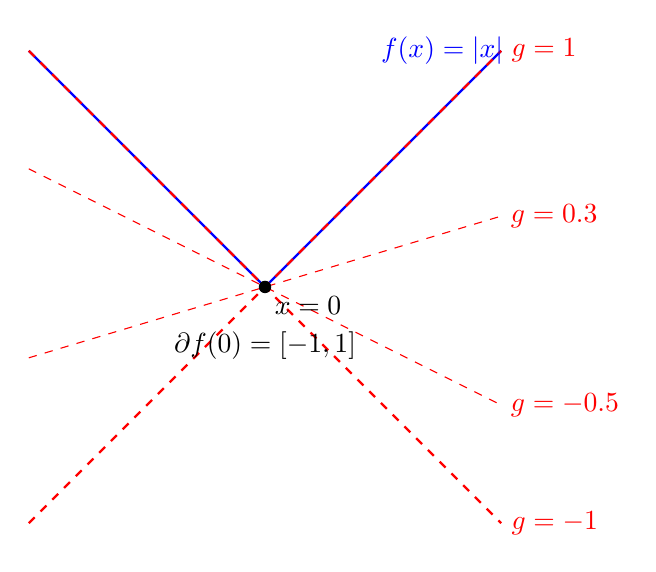
\begin{tikzpicture}[scale=1.5]
    % Function |x|
    \draw[thick, blue, domain=-2:0] plot (\x, {-\x});
    \draw[thick, blue, domain=0:2] plot (\x, {\x});

    % Subgradients at x=0
    \draw[red, dashed, domain=-2:2] plot (\x, {-0.5*\x}) node[right] {$g = -0.5$};
    \draw[red, dashed, domain=-2:2] plot (\x, {0.3*\x}) node[right] {$g = 0.3$};
    \draw[red, thick, dashed, domain=-2:2] plot (\x, {-\x}) node[right] {$g = -1$};
    \draw[red, thick, dashed, domain=-2:2] plot (\x, {\x}) node[right] {$g = 1$};

    \fill[black] (0,0) circle (1.5pt) node[below right] {$x = 0$};
    \node[blue] at (1.5, 2) {$f(x) = |x|$};
    \node at (0, -0.5) {$\partial f(0) = [-1, 1]$};
\end{tikzpicture}
\end{center}

\section{Impl\'ementation Python}

\begin{codeblock}[title=\textbf{M\'ethode du sous-gradient pour la norme $\ell_1$}]
\begin{minted}{python}
import numpy as np
import matplotlib.pyplot as plt

def subgradient_l1(A, b, x0, n_iter=500, c=1.0):
    """Minimise ||Ax - b||_1 par sous-gradient."""
    x = x0.copy()
    n = len(x)
    f_best = np.inf
    x_best = x.copy()
    history = []

    for k in range(n_iter):
        r = A @ x - b
        f_val = np.sum(np.abs(r))
        if f_val < f_best:
            f_best = f_val
            x_best = x.copy()
        history.append(f_best)

        # Sous-gradient de ||Ax - b||_1
        g = A.T @ np.sign(r)
        # Pas de Polyak-like
        alpha = c / np.sqrt(k + 1)
        x = x - alpha * g

    return x_best, history

# Test
np.random.seed(42)
m, n = 50, 20
A = np.random.randn(m, n)
x_true = np.zeros(n)
x_true[:5] = np.random.randn(5)
b = A @ x_true + 0.1 * np.random.randn(m)

x0 = np.zeros(n)
x_sol, hist = subgradient_l1(A, b, x0, n_iter=1000)

plt.semilogy(hist)
plt.xlabel('Iteration')
plt.ylabel('Best f value')
plt.title('Subgradient method for L1 minimization')
plt.grid(True, alpha=0.3)
plt.savefig('subgradient_l1.pdf')
\end{minted}
\end{codeblock}

\section{Exercices}

\begin{exercice}[$\star$]
Calculer le sous-diff\'erentiel de $f(x) = \max(0, x)$ en tout point $x \in \R$.
\end{exercice}

\begin{exercice}[$\star$]
Calculer $\partial f(x)$ pour $f(x) = \norm{x}_2$ sur $\R^n$.
\end{exercice}

\begin{exercice}[$\star\star$]
Soit $f(x) = \max(x_1, x_2)$ sur $\R^2$. Calculer $\partial f(x)$ pour
$(x_1, x_2)$ avec $x_1 > x_2$, $x_1 < x_2$, et $x_1 = x_2$.
\end{exercice}

\begin{exercice}[$\star\star$]
Montrer la r\`egle de somme~: si $f$ et $g$ sont convexes avec
$\mathrm{dom}(f) \cap \mathrm{int}(\mathrm{dom}(g)) \neq \emptyset$,
alors $\partial(f+g)(x) = \partial f(x) + \partial g(x)$.
\end{exercice}

\begin{exercice}[$\star\star$]
Montrer que le c\^one normal $N_C(x) = \partial \iota_C(x)$ est un c\^one convexe ferm\'e.
\end{exercice}

\begin{exercice}[$\star\star\star$]
Montrer que $f$ est convexe si et seulement si l'op\'erateur $\partial f$ est monotone.
\end{exercice}

\begin{exercice}[$\star\star\star$]
Impl\'ementer la m\'ethode du sous-gradient avec pas de Polyak pour minimiser
$f(x) = \norm{Ax - b}_1 + \lambda\norm{x}_\infty$ et comparer avec CVXPY.
\end{exercice}
